Deep networks are commonly used to model dynamical systems, predicting how the state of a system will evolve over time (either autonomously or in response to control inputs). Despite the predictive power of these systems, it has been difficult to make formal claims about the basic properties of the learned systems. In this chapter, we propose an approach for learning dynamical systems that are guaranteed to be stable over the entire state space. The approach works by jointly learning an unconstrained dynamics model and Lyapunov function, then combining them in a novel reprojection layer to produce models that are guaranteed to be stable by construction everywhere in the state space, even without any training. We show that such learning systems are able to model dynamical systems such as compound pendulums and can be combined with additional deep generative models to learn ro generate images with complex dynamics such as video textures.

\emph{From ``Learning Stable Deep Dynamics Models'' by \citeauthor{manek2019stable} (\citeyear{manek2019stable})}

\clearpage

\section{Introduction}

This chapter deals with the task of learning continuous-time dynamical systems. Given $x(t) \in \mathbb{R}^n$, a state at time $t$, we wish to model the time-derivative
\begin{align}
	\dot{x}(t) \equiv \frac{d}{dt}x(t) = f(x(t))
\end{align}
for some function $f : \mathbb{R}^n \rightarrow \mathbb{R}^n$. Modeling the time evolution of such dynamical systems (or with control inputs $\dot{x}(t) = f(x(t),u(t))$ for $u(t) \in \mathbb{R}^m$ and $f : \mathbb R^n \times \mathbb R^m \to \mathbb R^n$) is a foundational problem in machine learning, with applications in reinforcement learning, control, forecasting, and many other settings. Owing to their representational power, neural networks have long been a natural choice for modeling the function $f$ \citep{gu2016continuous,nagabandi2018neural,mishra2017prediction,gal2016improving}. However, when using a neural network to model dynamics in this setting very little can be guaranteed about the behavior of the learned system, especially about its stability. Informally, we say that a model is stable if we can pick a bounded set of states and guarantee that once the model enters that set it never leaves.  While some recent work has begun to consider stability properties of neural networks \citep{chow2018lyapunov,richards2018lyapunov,taylor2019episodic}, it has typically done so by softly enforcing stability as an additional loss term on the training data. Consequently, they can say little about the stability of the system in states outside the training data.

In this chapter, we propose an approach to learning neural network dynamics that are provably Lyapunov-stable over the entirety of the state space. We do this by jointly learning a nominal system dynamics and the certifying Lyapunov function, and then reprojecting the predictions of the nominal model onto the level set of the Lyapunov function. This stability is a hard constraint imposed upon the model: unlike recent approaches, we do not enforce stability via an imposed loss function but build it directly into the dynamics of the model. This means that even a randomly initialized model in our proposed model class will be provably stable everywhere in state space. The key to this is the design of a proper Lyapunov function, based on input convex neural networks \citep{amos2017input}, which ensures global exponential stability to an equilibrium point while still allowing for rich dynamics.

Using these methods, we demonstrate learning dynamics of physical models such as $n$-link pendulums, and show a substantial improvement over generic networks.  We also show how such dynamics models can be integrated into larger network systems to learn dynamics over complex output spaces, combining the model with a variational auto-encoder (VAE) \citep{kingma2013auto} to learn dynamic video textures \citep{schodl2000video}.

\section{Background and related work}

\paragraph{Stability of dynamical systems.} We consider the setting of uncontrolled\footnote{We will discuss extending this to dynamics with control later; this is a non-trivial extension.} dynamics systems $\dot{x}(t) = f(x(t))$ for $x(t) \in \mathbb{R}^n$. Such a system is \emph{globally asymptotically stable} around the equilibrium point $x_e=0$ if we have $x(t) \rightarrow 0$ as $t \rightarrow \infty$ for any initial state $x(0) \in \mathbb{R}^n$; $f$ is \emph{locally asymptotically stable} if the same holds but only for $x(0) \in \mathcal B$ where $\mathcal B$ is some bounded set containing the origin.  Similarly, $f$ is \emph{globally} or \emph{locally} exponentially stable if trajectories approach to the origin is at some minimum rate:
\begin{align}
	\|x(t)\|_2 \leq m \|x(0)\|_2 \, e^{-\alpha t}
\end{align}
for some constants $m, \alpha \geq 0$ for any $x(0) \in \mathbb{R}^n$ ($\mathcal B$, respectively).

The area of Lyapunov theory \citep{khalil2002nonlinear,la2012stability} establishes the connection between these types of stability according to a \emph{Lyapunov function}.  Specifically, let $V : \mathbb{R}^n \rightarrow \mathbb{R}$ be a continuously differentiable positive definite function, i.e., $V(x) > 0$ for $x \neq 0$ and $V(0) = 0$.  Lyapunov analysis says that $f$ is asymptotically stable, if and only if there exists some function $V$ as above such the value of this function decreases along trajectories generated by $f$.  Formally, this is the condition that the time derivative $\dot{V}(x(t)) < 0$, i.e.,
\begin{align}
	\dot{V}(x(t)) \equiv \frac{d}{dt}V(x(t)) = \nabla V(x)^T \frac{d}{dt} x(t) = \nabla V(x)^T f(x(t)) < 0
\end{align}
This condition must hold for all $x(t) \in \mathbb{R}^n$ or for all $x(t) \in \mathcal B$ to ensure global or local stability respectively.  Similarly $f$ is globally exponentially stable if and only if there exists positive definite $V$ with a sufficiently steep gradient such that
\begin{align}
	\dot{V}(x(t)) \leq -\alpha V(x(t)), \;\; \mbox{ with } c_1 \|x\|_2^2 \leq V(x) \leq c_2 \|x\|_2^2. \label{eqn:req_for_GAS}
\end{align}
Showing that these conditions imply the various forms of stability is relatively straightforward, but it is also true (but more complex to show) that any stable system must obey this property for some $V$.  In this chapter our broad stategy is to construct a Lyapunov function and enforce conditions that ensure stability.

\paragraph{Stability of linear systems. }
For a linear system with matrix $A$
\begin{align}
	\dot{x}(t) = A x(t)
\end{align}
it is well-known that the system is stable if and only if the real components of the the eigenvalues of $A$ are all strictly negative.  Equivalently, the same same property can be shown via a positive definite quadratic Lyapunov function
\begin{align}
	V(x) = x^T Q x
\end{align}
for $Q\in\mathbb R^{n\times n}, Q\succ 0$.  In this case, by Equation~\ref{eqn:req_for_GAS}, the following ensures global exponential stability:
\begin{align}
	\dot{V}(x(t)) = x(t)^T A^T Q x(t) + x(t)^T Q A x(t) \leq -\alpha x(t)^T Q x(t)
\end{align}
i.e., if we can find a positive definite matrix $Q \succeq I$ such that $A^T Q + Q A + \alpha Q \preceq 0$ negative semidefinite.  Such bounds (and much more complex extensions) for the basis for using linear matrix inequalities (LMIs), as a method to ensure stability of linear dynamical systems.  The methods also have applicability to non-linear systems, and several authors have used LMI analysis to learn non-linear dynamical systems by constraining the linearized systems to have global Lyapunov functions \cite{khansari2011learning,blocher2017learning,umlauft2017learning},

Even though the constraints
\begin{align}
	Q \succeq I, \;\; A^T Q + Q A + \alpha Q \preceq 0
\end{align}
are convex in $A$ and $Q$ separately, they are not convex in $A$ and $Q$ jointly.  Thus, the problem of jointly learning a stable linear dynamical system and its corresponding Lyapunov function, even for the simple linear-quadratic setting, is \emph{not} a convex optimization problem, and alternative techniques such as alternating minimization need to be employed instead.  Past work has considered different heuristics, such as approximately projecting a dynamics function $A$ onto the (non-convex) stable set of matrices with eigenvalues $\mathsf{Re}(\lambda_i(A)) < 0$ \citep{boots2008constraint}. It is no surprise, then, that learning stable non-linear systems is even more challenging:


\paragraph{Stability of non-linear systems}  For general non-linear systems, establishing stability via Lyapunov techniques is even more challenging.  For the typical task here, which is that of establishing stability of some \emph{known} dynamics $\dot{x}(t) = f(x(t))$, finding a suitable Lyapunov function is often more an art than a science.  Although some general techniques such as sum-of-squares certification \citep{parrilo2000structured,papachristodoulou2002construction} provide methods for certifying stability of polynomial (or similar) systems, these are often expensive and don't easily scale to high dimensional systems.
Our proposed approach here is able to learn provably stable systems without solving this generally hard problem.  While it is difficult to find a Lyapunov function that certifies the stability of some \emph{known} system, we exploit the fact that it is relatively much easier to \emph{enforce} some function to behave in a stable manner according to a Lyapunov function.

\paragraph{Lyapunov functions in deep learning}
Finally, there has been a small set of recent work exploring the intersection of deep learning and Lyapunov analysis \citep{chow2018lyapunov,richards2018lyapunov,taylor2019episodic}.  Although related to our work here, the approach in this past work is quite different.  As is more common in the control setting, these papers try to learn neural-network-based Lyapunov functions for control policies, but in way that enforces stability via a loss penalty.  For instance Richards et al., \citep{richards2018lyapunov} optimize a loss function that encourages $\dot{V}(x) \leq 0$ for $x$ in some training set.  In contrast, our work guarantees stability everywhere in the state space, not just at a small set of points; but only for a simpler setting where the entire dynamics are to be learned (and hence can be `constrained to be stable) rather than a stabilizing controller for known dynamics.

\section{Joint learning of dynamics and Lyapunov functions}

The intuition of the approach we propose in this paper is straightforward: instead of learning a dynamics function and attempting to separately verify its stability via a Lyapunov function, we propose to jointly learn a dynamics model and Lyapunov function, where the dynamics is inherently constrained to be stable (everywhere in the state space) according to the Lyapunov function.

Specifically, following the principles mentioned above, let $\hat{f} : \mathbb{R}^n \rightarrow \mathbb{R}^n$ denote a ``nominal'' unconstrained dynamics model, and let $V : \mathbb{R}^n \rightarrow \mathbb{R}$ be a positive definite function: $V(x) \geq 0$ for $x \neq 0$ and $V(0) = 0$.  Then in order to (provably, globally) ensure that a dynamics function is stable, we can simply project $\hat{f}$ such that it points down the gradient of the Lyapunov function. This corresponds to the condition
\begin{align}
	\nabla V(x)^T \hat{f}(x) \leq -\alpha V(x)
\end{align}
i.e., we define the dynamics
\begin{align}
	\label{eq:dynamics}
	\begin{split}
		f(x) & =  \mathsf{Proj}\left(\hat{f}(x), \{f: \nabla V(x)^T f \leq -\alpha V(x)\}\right) \\
		& = \begin{cases} \hat{f}(x) & \mbox{if } \nabla V(x)^T \hat{f}(x) \leq -\alpha V(x) \\
              \hat{f}(x) - \frac{\nabla V(x)}{\|\nabla V(x)\|_2^2} \left(\nabla V(x)^T \hat{f}(x) + \alpha V (x)\right)
                         & \mbox{otherwise}\end{cases} \\
		& = \hat{f}(x) - \frac{\nabla V(x)}{\|\nabla V(x)\|_2^2} {\mathsf{ReLU}\bigl(\nabla V(x)^T \hat{f}(x) + \alpha V (x) \bigr)}
	\end{split}
\end{align}
where $\mathsf{Proj(x;\mathcal{C})}$ denotes the orthogonal projection of $x$ onto the point $\mathcal{C}$, and where the second equation follows from the analytical projection of a point onto a half-space.  As long as $V$ is defined using automatic differentiation tools, it is straightforward to include the gradient $\nabla V$ terms into the definition of $f$, and our final network can be trained just like any other function.   The general approach here is illustrated in Figure \ref{fig:stable_nn_construction}.


\begin{figure}
    \centering
    \begin{tikzpicture}
        \begin{groupplot}[
                group style={
                        group name=my plots,
                        group size=4 by 1,
                        ylabels at=edge left,
                        yticklabels at=edge left,
                        horizontal sep=12pt
                    },
                axis on top,% ----
                width=1.3in,
                height=1.3in,
                scale only axis,
                enlargelimits=false,
                xmin=0,
                xmax=1,
                ymin=0,
                ymax=1,
                yticklabels={,,},
                xticklabels={,,}
            ]

            \nextgroupplot[title={Trajectory and Lyapunov function}]
            \addplot[] graphics[xmin=0,ymin=0,xmax=1,ymax=1] {LSDDM/figures/explanation/process-components.png};
            \node[anchor=west] (A) at (axis cs:0.1,0.85){\textbullet $x_e$};
            \node (B) at (axis cs:0.65,0.2){increasing $V$};
            \draw[->](A)--(B);
            \node[anchor=north] (C) at (axis cs:0.705,0.64){\textbullet $ x$};

            \nextgroupplot[title={Case 1}]
            \addplot[] graphics[xmin=0,ymin=0,xmax=1,ymax=1] {LSDDM/figures/explanation/process-components.png};
            \node[anchor=north] (C) at (axis cs:0.705,0.64){\textbullet \phantom{$ x$}};
            \node[inner sep=0pt] (A) at (axis cs:0.67,0.6){};
            \node[inner sep=2pt] (B) at (axis cs:0.7,0.1){};
            \draw [->] (A) -- node [midway,right] {$\hat f( x)$} (B);
            \node[inner sep=2pt] (D) at (axis cs:0.4,0.34){};
            \draw [->] (B) -- node [midway,left] {$-g( x)$} (D);
            \draw [->] (A) -- node [midway,left] {$f( x)$} (D);

            \nextgroupplot[title={Case 2}]
            \addplot[] graphics[xmin=0,ymin=0,xmax=1,ymax=1] {LSDDM/figures/explanation/process-components.png};
            \node[anchor=north] (C) at (axis cs:0.705,0.64){\textbullet \phantom{$ x$}};
            \node[inner sep=0pt] (A) at (axis cs:0.67,0.6){};
            \node[inner sep=2pt] (D) at (axis cs:0.4,0.55){};
            \node[inner sep=2pt] (E) at (axis cs:0.47,0.84){$g( x)$};
            \draw [->] (A) -- node [midway,below] {$f( x) = \hat f( x)$} (D);
            \draw [->] (A) -- (E);
        \end{groupplot}
    \end{tikzpicture}
    \caption{We plot the trajectory and the contour of a Lyapunov function of a stable dynamical system and illustrate our method. Let $g( x) = \frac{\nabla V(x)}{\|\nabla V(x)\|_2^2} \mathrm{ReLU}\left(\nabla V(x)^T \hat{f}(x) + \alpha V (x)\right)$. In the first case $\hat f( x)$ has a component $g( x)$ not in the half-space, which we subtract to obtain $f( x)$. In the second case $\hat f( x)$ is already in the half-space, so is returned unchanged.}
    \label{fig:stable_nn_construction}
\end{figure}


\subsection[Properties of the Lyapunov function]{Properties of the Lyapunov function $V$}\label{sec:lyapunov_properties}

Although the treatment above seems to make the problem of learning stable systems quite straightforward, the subtlety of the approach lies in the choice of the function $V$. Specifically, $V$ needs to be positive definite and needs to have no local optima except the global optimum at $0$. This is due to Lyapunov decrease condition: recall that we are attempting to guarantee stability to the equilibrium point $x=0$, yet the decrease condition imposed upon the dynamics means that $V$ is decreasing along trajectories of $f$.  If $V$ has a local optimum away from the origin, the dynamics may get stuck in this location; this manifests as the $\|\nabla V(x)\|_2^2$ term going to zero.

To enforce these conditions, we make the following design decisions regarding $V$:

\paragraph{No local optima.} We represent $V$ via an input-convex neural network (ICNN) function $g : \mathbb R^n \to \mathbb R$ \citep{amos2017input}, which enforces the condition that $g(x)$ be convex in its inputs $x$. Such a network is given by the recurrence
\begin{align}
	\begin{split}
		z_1 & = \sigma_0(W_0 x + b_0) \\
		z_{i+1} & = \sigma_i(U_i z_i + W_i x + b_i) \qquad i\in \{1,\ldots,k-1\} \\
		g(x) & \equiv z_k
	\end{split} . \label{eqn:icnnrecurrence}
\end{align}

For layer $i+1$: $W_i$ are weights mapping from the input $x$ to the $i+1$ layer activations; $U_i$ are positive weights mapping previously layer activations $z_i$ to the next layer; $b_i$ are real-valued biases; and $\sigma_i$ are convex, monotonically non-decreasing non-linear activations such as the ReLU or smooth variants. It is straightforward to show that with this formulation, $g$ is convex in $x$ \citep{amos2017input}, and indeed any convex function can be approximated by such networks \citep{chen2018optimal}.

\paragraph{Positive definite.} The ICNN property enforces that $V$ has only a single global optimum; for $V$ to be positive definite, we must also enforce that this optimum is at $x = 0$. We could fix this by removing the bias term from Equation~\ref{eqn:icnnrecurrence}, but this would mean we could no longer represent arbitrary convex functions. We could also shift whatever global minimum to the origin, but that would require finding finding the global minimum during training, which itself is computationally expensive. Instead, we take an alternative approach: we shift the function such that $V(0) = 0$, and add a small quadratic regularization term to ensure strict positive definiteness.
\begin{align}
	V(x) = \sigma_{k+1}(g(x) - g(0)) + \epsilon \|x\|_2^2.
	\label{eq:V_definition}
\end{align}
where $\sigma_k$ is a positive convex non-decreasing function with $\sigma_k(0) = 0$, $g$ is the ICNN defined previously, and $\epsilon$ is a small constant.  These terms together still enforce (strong) convexity and positive definiteness of $V$.

% \begin{comment}
\begin{figure}
    \centering
    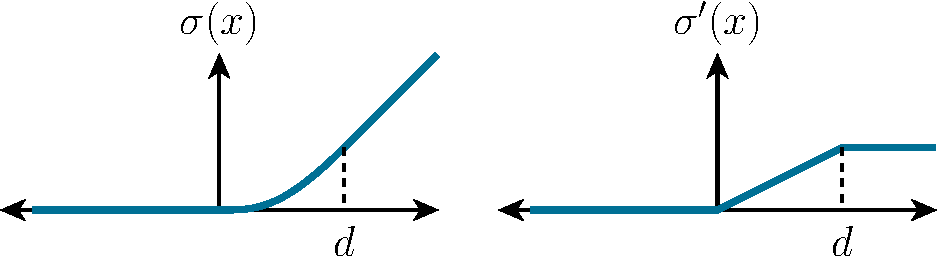
\includegraphics[width=.66\textwidth]{LSDDM/figures/rehu.pdf}
    \caption{Rectified Huber Unit (ReHU), necessary for continuously differentiable Lyapunov functions. }
    \label{fig:rehu}
\end{figure}
% \end{comment}

\paragraph{Continuously differentiable.}  Although not always required, several of the conditions for Lyapunov stability are simplified if $V$ is continuously differentiable. ReLU is discontinuous around 0, and the soft-plus smoothed ReLU is not zero at the origin. We use a smoothed version with quadratic knee in $[0, d]$, called the Rectified Huber Unit (ReHU):
\begin{align}
	\sigma(x) = \begin{cases} 0                   & \mbox {if } x \leq 0 \\
              \nicefrac{x^2}{2d}  & \mbox{if } 0 < x < d \\
              x - \nicefrac{d}{2} & \mbox{otherwise}\end{cases}.
\end{align}
An illustration of this activation is shown in Figure \ref{fig:rehu}.

\paragraph{Optionally warped input space. }  Our construction so far guarantees that the Lyapunov function has no local optima by making it convex. This is sufficient but not necessary, and it may even impose too strict a constraint on the learned dynamics. We can relax this function by allowing the input to the ICNN to be warped by any continuously differentiable invertible function $F : \mathbb{R}^n \times \mathbb{R}^n$. i.e., using
\begin{align}
	V(x) = \sigma_{k+1}(g(F(x)) - g(F(0))) + \epsilon \|x\|_2^2.
	\label{eq:V_definition2}
\end{align}
as the Lyapunov function.  Invertibility ensures that the level sets of $V$, which are convex, map to contiguous regions of the composite function $g \circ F$. This allows the resultant Lyapunov function to be non-convex without having any optima other than the global.

With these conditions in place, we have the following result.
\begin{theorem}
	The dynamics defined by
	\begin{align}
		\dot{x} = f(x)
	\end{align}
	are globally exponentially stable to the equilibrium point $x=0$. Where $f$ is from Eqn.~\ref{eq:dynamics} and $V$ is from Eqn.~\ref{eq:V_definition} or Eqn.~\ref{eq:V_definition2}, and $\hat{f}$ and $V$ functions have finite, bounded weights.
\end{theorem}
\begin{proof}
	The proof is straightforward, and relies on the properties of the networks created above.  First, note that by our definitions we have, for some $M$,
	\begin{align}
		\epsilon \|x\|^2_2 \leq V(x) \leq M \|x\|_2^2
	\end{align}
	where the lower bound follows from Eqn.~\ref{eq:V_definition} and the fact that $g$ is positive. The upper bound follows from the fact that the ReHU activation is linear for large $x$ and quadratic around 0.  This in turn implies that $V(x)$ behaves linearly as $\|x\|\rightarrow \infty$, and is quadratic around the origin, so can be upper bounded by some quadratic $M \|x\|_2^2$.

	The fact the $V$ is continuously differentiable means that $\nabla V(x)$ (in $f$) is defined everywhere, bounds on $\|\nabla V(x)\|_2^2$ for all $x$ follows from the the Lipschitz property of $V$, the fact that $0 \leq \sigma'(x) \leq 1$, and the $\epsilon \|x\|_2^2$ term
	\begin{align}
		\epsilon \|x\|_2 \leq  \|\nabla V(x)\|_2 \leq \sum_{i=1}^k \prod_{j=i}^k \|U_j\|_2 \|W_i\|_2
	\end{align}
	where $\|\cdot\|_2$ denotes the operator norm when applied to a matrix.  This implies that the dynamics are defined and bounded everywhere owing to the choice of function $\hat{f}$.

	Now, consider some initial state $x(0)$.  The definition of $f$ implies that
	\begin{align}
		\frac{d}{dt} V(x(t))  & = \nabla V(x)^T \frac{d}{dt} x(t) = \nabla V(x)^T f(x) \leq -\alpha V(x(t)).
		\intertext{Integrating this equation gives the bound}
		V(x(t))               & \leq V(x(0))e^{-\alpha t}
		\intertext{and applying the lower and upper bounds gives}
		\epsilon \|x(t)\|_2^2 & \leq M \|x(0)\|_2^2 e^{-\alpha t}
		\; \Longrightarrow \; \|x(t)\|_2 \leq \frac{M}{\epsilon} \|x(0)\|_2 e^{-\alpha t/2}
	\end{align}
	as required for global exponential convergence.
\end{proof}




\section{Empirical results}

We illustrate our technique on several example problems, first highlighting the inherent stability of the method for random networks, demonstrating learning on simple $n$-link pendulum dynamics, and finally learning high-dimensional stable latent space dynamics for dynamic video textures via a VAE model.

\subsection{Random networks}


\begin{figure}
    \centering
    \begin{tikzpicture}
        \begin{groupplot}[
                group style={
                        group name=my plots,
                        group size=4 by 1,
                        ylabels at=edge left,
                        yticklabels at=edge left,
                        horizontal sep=12pt
                    },
                axis on top,% ----
                width=1.33in,
                height=1.33in,
                scale only axis,
                enlargelimits=false,
                xmin=-2,
                xmax=2,
                ymin=-2,
                ymax=2,
            ]

            \nextgroupplot[title={Nominal $\hat f$}]
            \addplot[] graphics[xmin=-2,ymin=-2,xmax=2.2,ymax=2.2] {LSDDM/figures/random/fhat_dynamics.eps};
            \nextgroupplot[title={Lyapunov Function $V$}]
            \addplot[] graphics[xmin=-2,ymin=-2,xmax=2,ymax=2] {LSDDM/figures/random/V_lyap.eps};
            \nextgroupplot[axis equal image, axis lines=none, xtick=\empty, ytick=\empty]
            \addplotgraphicsnatural [xmin=-2, xmax=2, ymin=-2, ymax=2] {LSDDM/figures/pendulum/nn-lyapunov-cmap.eps};
            \nextgroupplot[title={Stable $f$}]
            \addplot[] graphics[xmin=-2,ymin=-2,xmax=2.2,ymax=2.2] {LSDDM/figures/random/f_dynamics.eps};
        \end{groupplot}
    \end{tikzpicture}
    \caption{(left) Nominal dynamics $\hat{f}$ for random network; (center) Convex positive definite Lyapunov function generated by random ICNN with constraints from Section \ref{sec:lyapunov_properties}; (right) Resulting stable dynamics $f$.}
    \label{fig:nominal_dynamics}
\end{figure}


As a powerful visualization of the fact that our model is stable by construction, we can plot the dynamics created by random networks, i.e., without any training at all. Because the dynamics models are inherently stable, these random networks lead to stable dynamics with interesting behaviors, illustrated in Figure \ref{fig:nominal_dynamics}.  Specifically, we let $\hat{f}$ be defined by a fully connected network and $V$ be an ICNN. Both networks have two hidden layers with 100 nodes each, and are initialized by the Kaiming uniform initialization \citep{he2015delving}. The $U$ weights in the ICNN are further subject to a softplus unit to make them positive.

\subsection[n-link pendulum]{$n$-link pendulum}

Next we look at the ability of our approach to model a dynamical system from kinematics, specifically the $n$-link pendulum.  A damped, rigid $n$-link pendulum's state $x$ can be described by the angular position $\theta_i$ and angular velocity $\theta_i$ of each link $i$.  As before $\hat f$ and the Lyapunov function $V$ have two hidden layers of 100 nodes, with properties described in Section~\ref{sec:lyapunov_properties}. Models are trained with pairs of data $(x, \dot x)$ produced by the symbolic algebra solver \texttt{sympy}, using simulation code adapted from \cite{vanderplas_2017}.


\begin{figure}
    \centering
    \begin{tikzpicture}
        \begin{groupplot}[
                group style={
                        group name=my plots,
                        group size=4 by 1,
                        ylabels at=edge left,
                        yticklabels at=edge left,
                        horizontal sep=18pt
                    },
                axis on top,% ----
                width=1.33in,
                height=1.33in,
                scale only axis,
                enlargelimits=false,
                xmin=-2,
                xmax=2,
                ymin=-2,
                ymax=2,
            ]

            \nextgroupplot[title={Simulated}]
            \addplot[] graphics[xmin=-2,ymin=-2,xmax=2,ymax=2] {LSDDM/figures/pendulum/true-stream.eps};
            \nextgroupplot[title={Learned $f$}]
            \addplot[] graphics[xmin=-2,ymin=-2,xmax=2,ymax=2] {LSDDM/figures/pendulum/nn-stream.eps};
            \nextgroupplot[title={Learned $V$}]
            \addplot[] graphics[xmin=-2,ymin=-2,xmax=2,ymax=2] {LSDDM/figures/pendulum/nn-lyapunov.eps};
            \nextgroupplot[axis equal image, axis lines=none, xtick=\empty, ytick=\empty]
            \addplotgraphicsnatural [xmin=-2, xmax=2, ymin=-2, ymax=2] {LSDDM/figures/pendulum/nn-lyapunov-cmap.eps};
        \end{groupplot}
    \end{tikzpicture}
    \caption{Dynamics of a simple damped pendulum. From left to right: the dynamics as simulated from first principles, the dynamics model $f$ learned by our method, and the Lyapunov function $V$ learned by our method (under which $f$ is non-expansive).}
    \label{fig:pendulum_experiment}
\end{figure}{}


In Figure~\ref{fig:pendulum_experiment}, we compare the simulated dynamics with the learned dynamics in the case of a simple damped pendulum (i.e. with $n=1$), showing both the vector field and a single simulated trajectory, and draw a contour plot of the learned Lyapunov function. As seen, the system is able to learn dynamics that can accurately predict motion of the system even over long time periods. We can also recover the laws of conservation of energy implicit in the data, including the fact that kinetic energy is lost slowly but not potential energy.

\pgfplotstableread{LSDDM/figures/pendulum_results/nlinkerror_simple.dat}{\nlinkerrorsimple}
\pgfplotstableread{LSDDM/figures/pendulum_results/nlinkerror_rehu.dat}{\nlinkerrorrehu}
\pgfplotstableread{LSDDM/figures/pendulum_results/8_simple.dat}{\pendressimple}
\pgfplotstableread{LSDDM/figures/pendulum_results/8_REHU_0.005.dat}{\pendressrehu}
\pgfplotstableread{LSDDM/figures/pendulum_results/8_lstm.dat}{\pendresslstm}

\begin{figure}
    \begin{center}
        \begin{tikzpicture}
            \begin{groupplot}[
                    group style={
                            group name=my plots,
                            group size=2 by 1,
                            ylabels at=edge left,
                            yticklabels at=edge left,
                            horizontal sep=12pt
                        },
                    axis on top,% ----
                    height=1.2in,
                    width=2.35in,
                    scale only axis,
                    enlargelimits=false,
                    ymode=log
                ]

                \nextgroupplot[title={\shortstack{Error at each time\\ for 8-link pendulums}},
                    axis on top,% ----
                    scale only axis,
                    enlargelimits=false,
                    xmin=0, xmax=1000, ymin=100, ymax=100000,
                    ylabel near ticks,
                    legend pos=north west,
                    xlabel={Timestamp},
                    ylabel={Error}]

                \addplot+[]
                table [x={t}, y={loss}] {\pendressimple};
                \addplot+[]
                table [x={t}, y={loss}] {\pendressrehu};
                \legend{Simple,Stable}

                \nextgroupplot[title={\shortstack{Average error over 999 timesteps\\ for $n$-link pendulums}},
                    xmin=0.5, xmax=8.5,
                    ymin=10000, ymax=100000000,
                    xlabel={Number of links $n$}, xtick=data]
                \addplot+[] table [x={n}, y={loss}] {\nlinkerrorsimple};
                \addplot+[] table [x={n}, y={loss}] {\nlinkerrorrehu};

            \end{groupplot}
        \end{tikzpicture}
    \end{center}

    \caption{Error in predicting $
            \theta, \dot \theta$ in 8-link pendulum at each timestep (left); and average error over 999 timesteps as the number of links in the pendulum increases (right).}
    \label{fig:pendulum_results}
\end{figure}


We also evaluate the learned dynamics quantitatively varying $n$ and the time horizon of simulation. Figure~\ref{fig:pendulum_results} presents the total error over time for the 8-link pendulum, and the average cumulative error over 1000 time steps for different values of $n$.  While both the simple and stable models show increasing mean error at the start of the trajectory, our model is able to capture the loss of energy in the physical system and in fact exhibits decreasing error towards the end of the simulation. In comparison, the error in the simple model increases.

\subsection{Video Texture Generation}

Finally, we apply our technique to stable video texture generation, using a Variational Auto-Encoder (VAE) \citep{kingma2013auto} to learn an encoding for images, and our stable network to learn a dynamics model in the latent space.  Given a sequence of frames $(y_0, y_1, \ldots)$, we feed the network the frame at current time $t$
and train it to reconstruct the frames at the current time $t$ and subsequent time-step $t+1$. Specifically, we consider a VAE defined by the encoder $e : \mathcal{Y} \rightarrow \mathbb{R}^{2n}$ giving mean and variance $\mu, \log \sigma^2_t = e(y_t)$, latent state $z_t \in \mathbb{R}^n \sim \mathcal{N}(\mu_t, \sigma_t^2)$, and decoder $d: \mathbb{R}^n \rightarrow \mathcal{Y}$, $y_t \approx d(z_t)$.  We train the network to minimize both the standard VAE loss (reconstruction error plus a KL divergence term), but \emph{also} minimize the reconstruction loss of a next predicted state. We model the evolution of the latent dynamics at $z_{t+1} \approx f(z_t)$, or more precisely $y_{t+1} \approx d(f(z_t))$.  In other words, as illustrated in Figure~\ref{fig:vae_training}, we train the full system to minimize
\begin{align}
	\minimize_{e,d,\hat{f},V} \sum_{t=1}^{T-1} \biggl ( \mathsf{KL}(\mathcal{N}(\mu_t,\sigma_t^2 I\|\mathcal{N}(0,I)) + \mathbf{E}_z \bigl [ \|d(z_t) - y_t\|_2^2 + \| d(f(z_t)) - y_{t+1}\|_2^2 \bigr ] \biggr )
\end{align}



\begin{figure}
    \begin{tikzpicture}
        \begin{axis}[
                axis on top,% ----
                scale only axis,
                enlargelimits=false,
                xmin=0, ymin=0,
                xmax=527.577, ymax=134.747,
                width=5.5in,
                height=1.404in,
                yticklabels={,,},
                xticklabels={,,},
                axis line style={draw=none},
                tick style={draw=none}]
            \addplot[] graphics[xmin=0, ymin=0, xmax=527.577, ymax=134.747] {LSDDM/figures/vidtex-2/model-training-blank.png};
            \node (A) [anchor=north] at (axis cs:40,74){$e(y_t)$};
            \node (D) [anchor=south west] at (axis cs:66,102){$\mu_t$};
            \node (E) [anchor=north west] at (axis cs:66,82){$\log\sigma_t$};
            \node (H) [anchor=south west] at (axis cs:160,64){\small{$\hat f(z_t)$}};
            \node (H) [anchor=south west] at (axis cs:160,28){\small{$V(z_t)$}};
            \node (F) [anchor=south] at (axis cs:196,92){$z_t \in \mathcal{N}(\mu_t,\sigma_t^2)$};
            \node (J) [anchor=south] at (axis cs:286,35){\footnotesize{$z_{t+1} \gets z_t + f(z_t)$}};
            \node (B) [anchor=north east] at (axis cs:392,72){\footnotesize{$d(z_t)$}};
            \node (B) [anchor=north east] at (axis cs:392,20){\footnotesize{$d(z_{t+1})$}};
            \node (I) [anchor=west] at (axis cs:380,118){{KL}($\mathcal{N}(\mu_t,\sigma_t^2)\| \mathcal{N}(0,I))$};
            \node (K) [anchor=west] at (axis cs:396,82){$\|d(z_t) - y_{t}\|_2^2$};
            \node (K) [anchor=west] at (axis cs:396,28){$\|d(z_{t+1}) - y_{t+1}\|_2^2$};
        \end{axis}
    \end{tikzpicture}
    \caption{Structure of our video texture generation network. The encoder $e$ and decoder $d$ form a Variational Autoencoder, and the stable dynamics model $f$ is trained together with the decoder to predict the next frame in the video texture.}
    \label{fig:vae_training}
\end{figure}

\setlength{\tabcolsep}{2pt}
\newcommand{\sampletbl}[2]{
    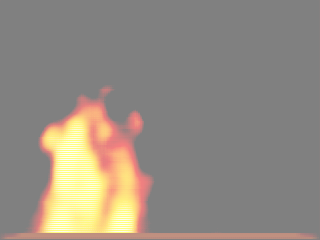
\includegraphics[width=0.4in]{LSDDM/figures/results/#1-#2/fr_00000.png} &
    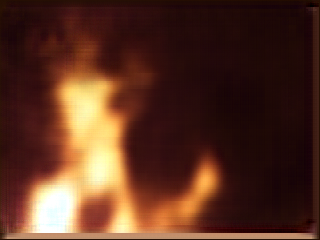
\includegraphics[width=0.4in]{LSDDM/figures/results/#1-#2/fr_00010.png} &
    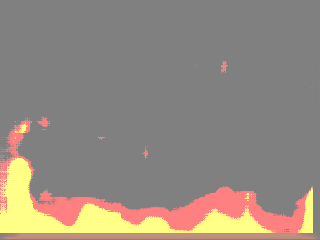
\includegraphics[width=0.4in]{LSDDM/figures/results/#1-#2/fr_00020.png} &
    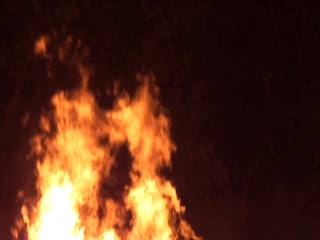
\includegraphics[width=0.4in]{LSDDM/figures/results/#1-#2/fr_00030.png} &
    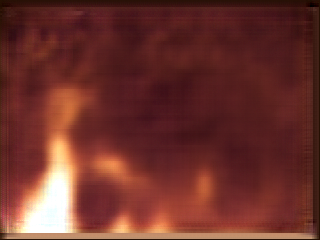
\includegraphics[width=0.4in]{LSDDM/figures/results/#1-#2/fr_00040.png} &
    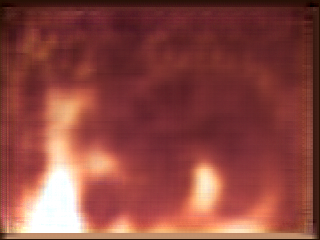
\includegraphics[width=0.4in]{LSDDM/figures/results/#1-#2/fr_00050.png}  &
    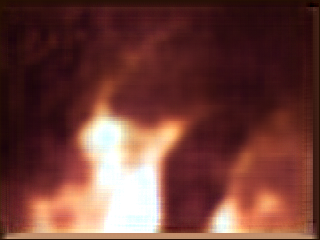
\includegraphics[width=0.4in]{LSDDM/figures/results/#1-#2/fr_00100.png} &
    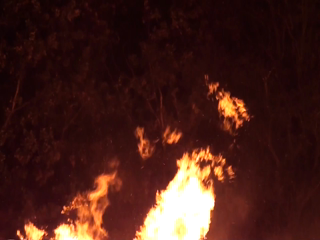
\includegraphics[width=0.4in]{LSDDM/figures/results/#1-#2/fr_00150.png} &
    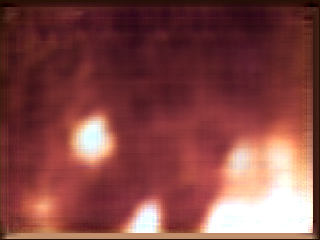
\includegraphics[width=0.4in]{LSDDM/figures/results/#1-#2/fr_00200.png} &
    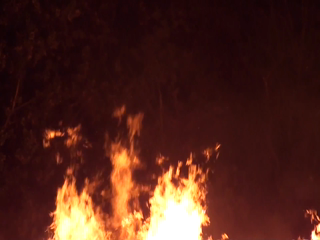
\includegraphics[width=0.4in]{LSDDM/figures/results/#1-#2/fr_00250.png}
}
\begin{figure}
    \centering
    \begin{tikzpicture}
        \begin{groupplot}[
                group style={
                        group name=my plots,
                        group size=5 by 1,
                        horizontal sep=12pt
                    },
                axis on top,% ----
                width=1.in,
                height=1.in,
                scale only axis,
                enlargelimits=false,
                xmin=0,
                xmax=1,
                ymin=0,
                ymax=1,
                axis x line*=bottom, axis y line*=left,
            ]

            \nextgroupplot[title={Stable Model Run 1},
                ytick={.1, 1},
                yticklabels={-2,18},
                xtick={.15, 1},
                xticklabels={$-10$,15}]
            \addplot[
                yticklabels={,,},
                xticklabels={,,}] graphics[xmin=-0.17,ymin=-0.17,xmax=1.17,ymax=1.17] {LSDDM/figures/results/bonfire-exp27r-1e-5-1231132/trajmodel.png};

            \nextgroupplot[title={Stable Model Run 2},
                ytick={.1, 1},
                yticklabels={0,$20$},
                xtick={.15, 1},
                xticklabels={$0$,25}]
            \addplot[] graphics[xmin=-0.17,ymin=-0.17,xmax=1.17,ymax=1.17] {LSDDM/figures/results/bonfire-exp27r-1e-5-1238886/trajmodel.png};

            \nextgroupplot[title={Stable Model Run 3},
                ytick={.1, 1},
                yticklabels={-10,8},
                xtick={.1, .8},
                xticklabels={-5,15}]
            ]
            \addplot[] graphics[xmin=-0.17,ymin=-0.17,xmax=1.17,ymax=1.17] {LSDDM/figures/results/bonfire-exp27r-1e-5-main/trajmodel.png};

            \nextgroupplot[title={Naive Model},
                ytick={.1, 1},
                yticklabels={0,},
                xtick={.1, 1},
                xticklabels={$-2 \times 10^{30}$,0},
                extra y tick labels={$1.2 \times 10^{30}$},
                extra y ticks={1.0},
                extra y tick style={y tick label style={right, xshift=0.25em}},]
            \addplot[] graphics[xmin=-0.17,ymin=-0.17,xmax=1.17,ymax=1.17] {LSDDM/figures/results/bonfire-bad2/trajmodel.png};

            \nextgroupplot[
                ytick={0,1},
                yticklabels={0,300},
                ylabel={steps},
                width=.05in,
                axis line style={draw=none}, tick style={draw=none}, xticklabel=\empty, every axis y label/.style={at={(current axis.west)},rotate=90,yshift=-3mm,xshift=1mm},
                y tick label style={right, xshift=0.25em}]

            \addplot[] graphics[xmin=0,ymin=0,xmax=1,ymax=1] {LSDDM/figures/viridis.png};

        \end{groupplot}
    \end{tikzpicture}
    \begin{tabular}{r|cccccc|cccc}
        Stable & \multicolumn{10}{c}{Frame Number}                                                                                             \\
        Model  & $0$                                      & ${10}$ & ${20}$ & ${30}$ & ${40}$ & ${50}$ & ${100}$ & ${150}$ & ${200}$ & ${250}$ \\
        Run 1  & \sampletbl{bonfire}{exp27r-1e-5-main}                                                                                         \\
        Run 2  & \sampletbl{bonfire}{exp27r-1e-5-1231132}                                                                                      \\
        Run 3  & \sampletbl{bonfire}{exp27r-1e-5-1238886}                                                                                      \\
        \shortstack{Naive                                                                                                                      \\Model} &
        \sampletbl{bonfire}{bad2}
        % \\ \shortstack{Sample\\Video} &    \sampletbl{bonfire}{sample}
    \end{tabular}

    \caption{Samples generated by our stable video texture networks, with associated trajectories above. The true latent space is 320-dimensional; we project the trajectories onto a two-dimensional plane for display. For comparison, we present the video texture generated using an unconstrained neural network in place of our stable dynamics model.}
    \label{fig:vae_results}
\end{figure}


We train the model on pairs of successive frames sampled from videos. To generate video textures, we seed the dynamics model with the encoding of a single frame and numerically integrate the dynamics model to obtain a trajectory. The VAE decoder converts each step of the trajectory into a frame. In Figure~\ref{fig:vae_results}, we present sample stable trajectories and frames produced by our network. For comparison, we also include an example trajectory and resulting frames when the dynamics are modelled without the stability constraint (i.e. letting $f$ in the above loss be a generic neural network).  For the naive model, the dynamics quickly diverge and produce a static image, whereas for our approach, we are able to generate different (stable) trajectories that keep generating realistic images over long time horizons. We control the ``temperature'' of the generation process by adding controlled amounts of random noise to the system at each step.

\section{Conclusion}

We proposed a method for learning provably stable non-linear dynamical systems using neural networks. The approach jointly learns a convex positive definite Lyapunov function along with dynamics constrained to be stable according to these dynamics everywhere in the state space.  We show that these models can be integrated into other deep architectures such as VAEs, and learn complex latent space dynamics is a fully end-to-end manner.  Although we have focused here on the autonomous (i.e. uncontrolled) setting, the method opens several directions for future work, such as integration into dynamical systems for control or for model-based reinforcement learning settings.  Having stable dynamics as a neural-network primitive can be useful in many diverse contexts, and combining these stable systems with the representational power of deep networks offers a powerful tool in modeling dynamical systems.


\section{Adaptation to Stable Control and RL }

After the successes of our stable dynamics model, we attempted to extend it to also learn stable policies and value functions. The intuitive extension to this is to replace the dynamics model $\hat f$ with fixed (known) dynamics $\tilde f$ and a learnable policy network $\pi$. That is, we train to minimize:
\begin{align}
	\mathsf{ReLU}\bigl(\nabla V(x)^T \tilde{f}(x, \pi) + \alpha V (x) \bigr)
\end{align}
given traces from simulated dynamics. We also transformed the dynamics so that the goal state was positioned at the origin, choosing suitable transformations for the dynamics and Lyapunov functions. As required by the approach, we attempted to train it from trajectory samples to minimize the error over one step.

We were able to successfully learn stabilizing controllers for toy examples such as a simple damped pendulum and for the cartpole problem. Unfortunately, we were not able to learn a swing-up controller for either environment, or any type of controller for an Acrobot\footnote{A two-link pendulum with a single actuator in the middle joint. A pendulum with an actuator at the fixed joint is a Pendubot \cite{underactuated}.} or more complex locomotion tasks. We observed that the training would consistently fail in the same way: the nominal dynamics function would diverge to the point of uselessness, followed by the learned Lyapunov function collapsing to a trivial function.

This persists despite any amount of regularization, hyperparameter tuning, and even across a variety of environments. Contemporary efforts in the literature were similarly unable to scale this approach to locomotion tasks. The consistent failure of this method suggested that an underlying principle was being violated, and that regularization was not able to address that. We eventually investigated how the difference in distributions between the data used to train the purportedly stable controller and the policy the controller was attempting to learn, which led us to the work in the next chapter.
